\section*{Memory Management}

\subsection*{Main Memory}
MM is the only storage the CPU can access directly. \textbf{Speed:} CPU Registers > Cache > Main Memory.
\begin{description}
    % Main Memory Partitions: resident OS in high PA, user Ps usually in low pa
    \item[Base and limit registers] smallest legal mem. address + size. Define \textbf{Logical Address Space (LAS)} of a P (set of all LA's). P can only access mem inside LAS (otherwise trap $\rightarrow$ fatal error). Only OS can access all registers/mem. \\
    \item[Logical Address / Virtual Address] generated by CPU. visible to user. editable \\
    \item[Physical Address] only seen by Mem. Unit. does not change. \textbf{PAS} set of  all PAs correspoding to LAS \\
    \item[Address Binding] mapping instructions and data to mem addresses. 3 schemes/stages: (in red) \\
    \item[Memory Management Unit MMU] HW device, maps LA to PA during execution. $\rightarrow$ mapping methods (relocation register, contiguous paging) \\
    \item[Dynamic Loading]: routine not loaded in mem until called. all routines kept on disk. no special os support needed \textbf{Static Linking}: Libraries and program code combined by loader. \textbf{Dynamic Linking} happens during execution. useful for shared libraries (standard C lib.) DLL: dynamically linked libraries. \\ %NOTE: also see introduction
\end{description}

\subsection*{Contiguous Memory Allocation}
each P is contained in a single section of mem that is contiguous to the section containing the next P. \textbf{Memory Protection} through usage of Relocation \& limit registers. degree of multiprog. limited by nr of partitions.
\begin{description}
    \item[Dynamic Storage Allocation]: OS maintains list of allocated \& free partitions (\textbf{Holes}). First-fit (fastest), Best-fit (eq. to ff in storage-utilization, produces smallest leftover-hole), worst-fit ($\rightarrow$ largest leftover hole) \\
    \item[Internal Fragmentation]: physical mem organized into fixed-size blocks. happens if allocated mem larger than requested mem (internal to partition). \\
    \item[External Fragmentation]: Total Mem Space for requests exists, but is not contiguous. 50\% rule: 1/3 unusable. \textbf{Solutions} \textit{Compaction}: moving data, can be expensive, only possible with dynamic address relocation (during ex. time) \textit{Noncontinguous Allocation}: Strategy used in Paging \\
\end{description}

\subsection*{Paging}
\begin{tikzpicture}[remember picture,overlay]
    \node[xshift=81.5mm,yshift=-4.5mm] at (current page.west){%
    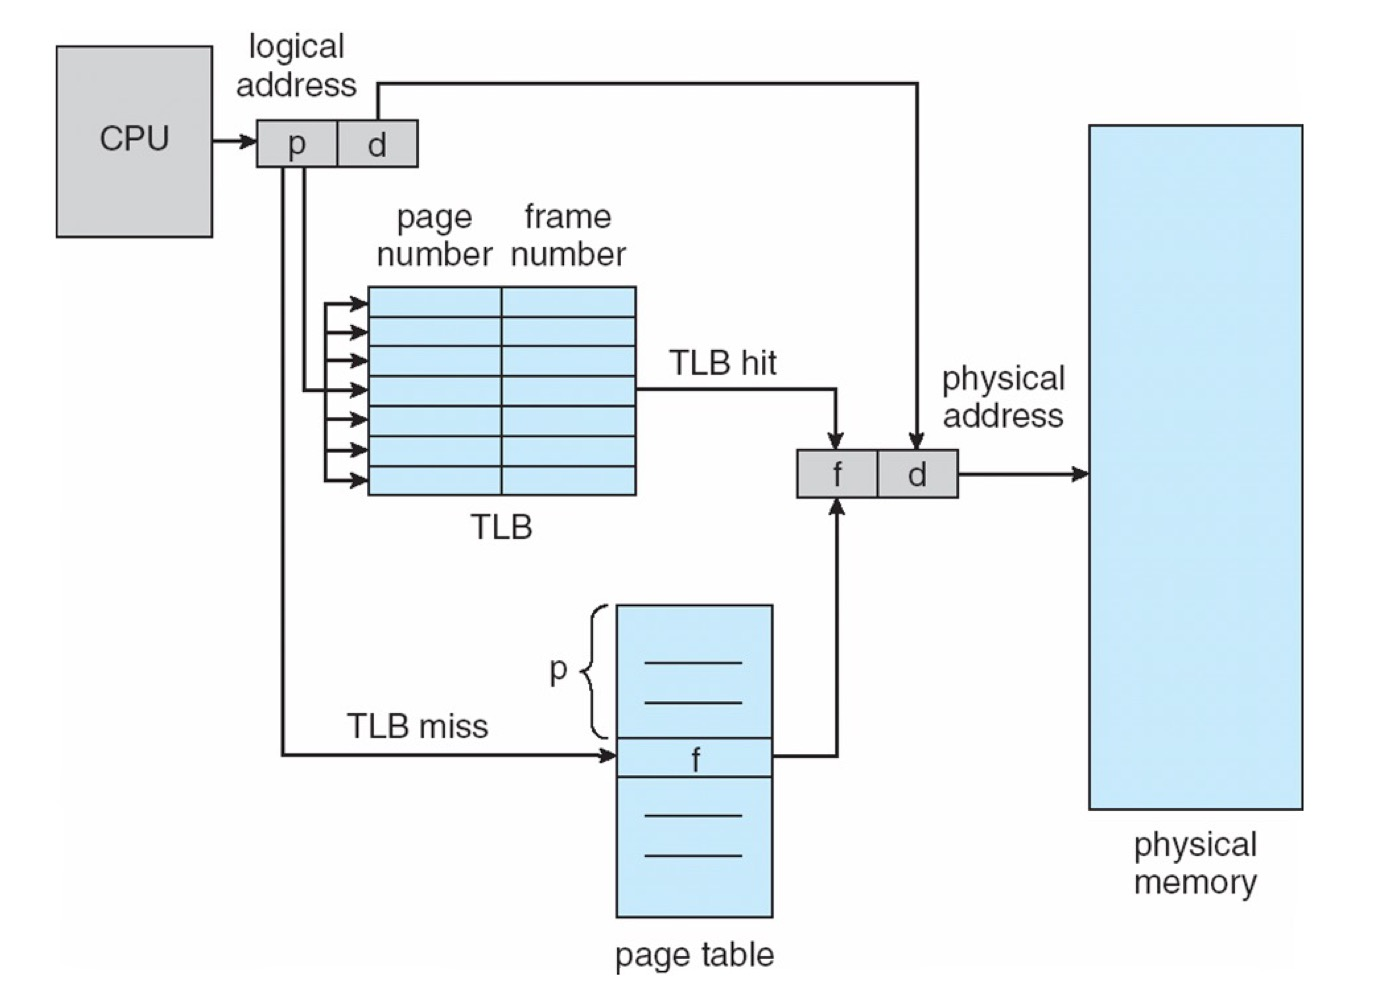
\includegraphics[width=40mm]{tlb.jpeg}};
\end{tikzpicture}
PA can be noncontiguous, mem for P allocated wherever possible (no ex. fragmentation, but some internal $\rightarrow$ smaller pages eq. less int. frag but move overhead in page table). Physical mem is divided into fixed-size blocks called \textbf{frames}. Logical mem divided into same-sized blocks called \textbf{pages}.\\
\begin{description}
    \item[Adress-Translation]: page number and page offset in the per-P page table
    \item[] OS keeps copy of each per-P page table + maintains frame table (for each physical frame)
    \item[Hardware Implementation]: per-P page table kept in main mem. \textbf{PTBR} page-table base register (pointers) \& \textbf{PTLR} page-table length register (size of page table)
    \item[Translation Lookaside Buffer TLB]: associative mem. hw cache for page table. (page nr, frame) \textbf{Replacement policies}: round-robin, LRU, random. key kernel code can be wired down for perm fast access
    \item[Memory Protection] protection bit (read-only, read-write) or valid-invalid bit (attached to each entry in the page table. indicates if legal (in LAS) or not)
    \item[Shared Pages]reentrant (unchanging) code shared among Ps. ex: std C lib
\item[Structure of the Page Table] mem structure overhead. ex: 32bit LAS \\
    Page Size 4KB ($2^{12}$), \# pages = $2^{20}$ $\rightarrow$ 1 mio entries in page table. \\
    \textbf{Solutions}: hashed page tables, inverted page tables
    \item[Hierarchical Page Table]ex: two-level, page the page table. (forward mapping) \\ %TODO: look at example
\end{description}
\vspace{5\baselineskip}
\subsection*{Swapping}
moving P temporarily out of mem to a \textit{backing store} and brought back for continued execution. (P roll out, roll in). system maintains ready queue. $\rightarrow$ transfer time too high, not used in modern OS
\begin{description}
    \item[Swapping with Paging]: pages of a P instead of whole P swapped. (page in, page out)
\end{description}
